\newpage
\section{Реализация}
\label{sec:Realization}

\subsection{Программные средства реализации}
Для разработки программной части приложения использовался высокоуровневый язык программирования Python версии 3.9.5. Программирование осуществлялось в редактор исходного кода Visual Studio Code~\cite{vscode}. 

\vspace{2em}
\subsection{Реализация компонентов приложения}
\label{subsec:Parser}
В данном разделе приводится описание реализации отдельных компонентов приложения. Код программной части представлен в репозитории на GitHub~\cite{github}.
\vspace{1em}

\textbf{Реализация модуля подготовки данных}

Исходными данными для этой работы служит статья о наборе данных GitHub~\cite{clickHouse}, содержащем информацию о всех событиях на этой платформе с 2011 года и насчитывающем более трех миллиардов записей. Данный набор данных был загружен в ClickHouse, который представляет собой открытую систему управления базами данных, специально разработанную для эффективного анализа и хранения больших объемов информации. 

Текущий датасет содержит множество полей, где каждая запись соответствует определенной действия, выполненной пользователем в одном из репозиториев. В частности, существует столбец <<event\_type>>, который описывает различные операции. Для данной работы имеют вес следующие операции: <<CommitCommentEvent>> (добавление коммита с комментарием), <<ForkEvent>> (создание форка репозитория), <<IssuesEvent>> (добавление обсуждения), <<PullRequestEvent>> (создание запроса на включение изменений), и <<WatchEvent>> (добавление звезды к проекту). В контексте работы с проектами, необходимо сгруппировать выполненные операции для каждого проекта. Следовательно, с использованием запросов можно получить информацию о названии проекта (репозитория) и количестве звезд, форков и других характеристик, связанных с данным репозиторием.

Помимо того, для демонстрации работы с общедоступными данными ClickHouse существует веб-страница, способная обрабатывать SELECT-запросы и предоставлять обширный объем информации. В силу того, что объем датасета более 80 ГБ, данные из него было решено получать с помощью веб-приложения, поэтому необходимо разработать способ, которым можно корректно их преобразовать.

Для реализации извлечения данных из датасета используется библиотека Selenium~\cite{selenium}, которая запускает имитацию использования браузера со вкладкой сайта в течение некоторого времени для выполнения запроса. Ждет время выполнения SQL-запроса в течение 15 секунд с помощью встроенной библиотеки time~\cite{time}. 

Парсинг веб-страницы и получение данных с сайта -- поиск необходимых элементов на веб-странице -- производится с помощью библиотеки Beautiful Soup~\cite{beautifulsoup}. 

Логику работы алгоритма получения данных с помощью HTML и таблицы из нее можно представить в виде диаграммы последовательности (рис.~\ref{ris:sequence}).

\begin{figure}[h]
    \centering
    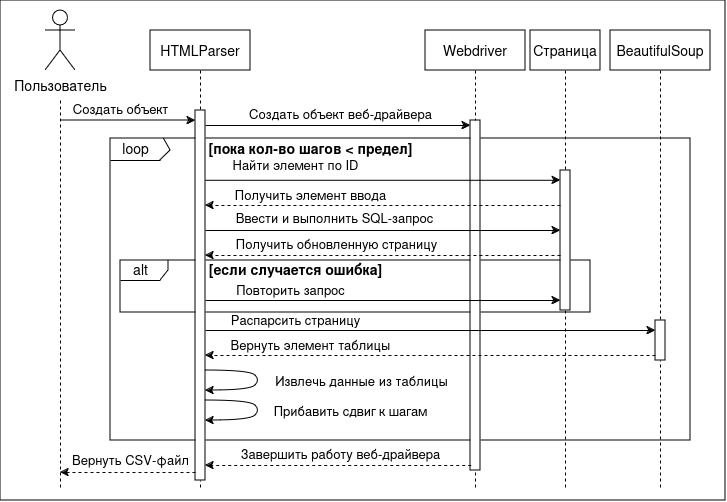
\includegraphics[width=1\linewidth]{pic/sequence.png}
    \vspace{0.2em}    \caption{Диаграмма последовательности}
    \label{ris:sequence}
\end{figure}
\vspace{1em}

В результате подготовки данных становятся доступны следующие данные о репозиториях: название, количество коммитов, пулл-реквестов, проблем, звезд, форков и участников. Для формирования и записи полученных результатов используется встроенная библиотека csv~\cite{csv}, позволяющая записывать результаты в CSV-файл.
\vspace{1em}

\textbf{Реализация модуля классификации}

Модуль классификации включает в себя определение класса популярности проекта, исходя из параметров репозиториев, и обучение моделей на основе данных csv-файла.

На вход приходит список, содержащий названия различных метрик (forks, commits, issues и т. д.), которые будут использоваться для вычисления общей метрики популярности проекта. Для вычисления общей метрики популярности берутся значения каждой метрики из списка metrics для каждого проекта в наборе данных. 

Вычисляются квантили для равномерного распределения по децилям -- на 10 классов популярностей. Вычисление квантилей применяется ко всем значениям общей метрики популярности и сохраняет результатов в наборе данных data. Таким образом, каждый проект получает свой собственный класс популярности на основе общей метрики популярности и квантилей.

С помощью библиотеки pandas~\cite{pandas} выполняется чтение данных из файла форма csv для дальнейшей обработки классов по значениям. 

Для обучения моделей использовались методы, функции и классы из библиотеки scikit-learn~\cite{sklearn}, которая  предоставляет широкий набор инструментов для машинного обучения и анализа данных с установкой необходимых параметров.
\vspace{1em}

\textbf{Реализация модуля регрессии}

Модуль регрессии выполняет прогнозирование значения звезд у репозиториев на основе остальных параметров.

На вход аналогично модулю классификации приходит набор данных со списком различных метрик. Основное отличие, что в данном случае целевой переменной является уже имеющееся значение звезд в наборе данных. На основе этих данных модель выделяет 20\% тестовых данных и 80\% данных для обучения. Реализован модуль с помощью класса GHregressor, который наследуется от IGHModel, имеющий абстрактные методы для предсказания результата, обучения модели и сохранения модели в файл или загрузки -- из файла. 

Метод загрузки и сохранения файла выполнен с помощью библиотеки joblib~\cite{joblib}, которая предоставляет инструменты для эффективного сохранения и загрузки объектов моделей.
\vspace{1em}

\textbf{Реализация модуля оценки работы моделей}

В рамках модуля оценки работы моделей реализован подсчет метрик машинного обучения и отображения результатов.

На вход приходит обученная ранее модель, способная предоставить информацию. Для моделей классификации ведется подсчет метрик F1, precision, recall и accuracy, для моделей регрессий -- MSE, MAE, $R^2$. Кроме того, имеется построение матрицы ошибок относительно данных в рамках моделей классификации, которые отображают верно выбранные результаты классов, а также сохранение матрицы ошибок в файл.

С помощью библиотеки scikit-learn~\cite{sklearn} получают результаты матрицы ошибок по обучению моделей и определению класса популярности данных.

Визуализация матриц ошибок выполяется с помощью библиотеки matplotlib~\cite{matplotlib}, а его модуль pyplot помогает создавать диаграмму,  позволяя при этом настроить его внешний вид. А получение и сортирование по критериям в рамках графика данных выполняется с помощью библиотеки seaborn~\cite{seaborn}.

Данную реализацию перечисленных модулей можно представить в виде диаграммы классов UML, которая представлена на рисунке~\ref{ris:uml}.
\vspace{1em}

\newpage
\begin{figure}[h]
    \centering
    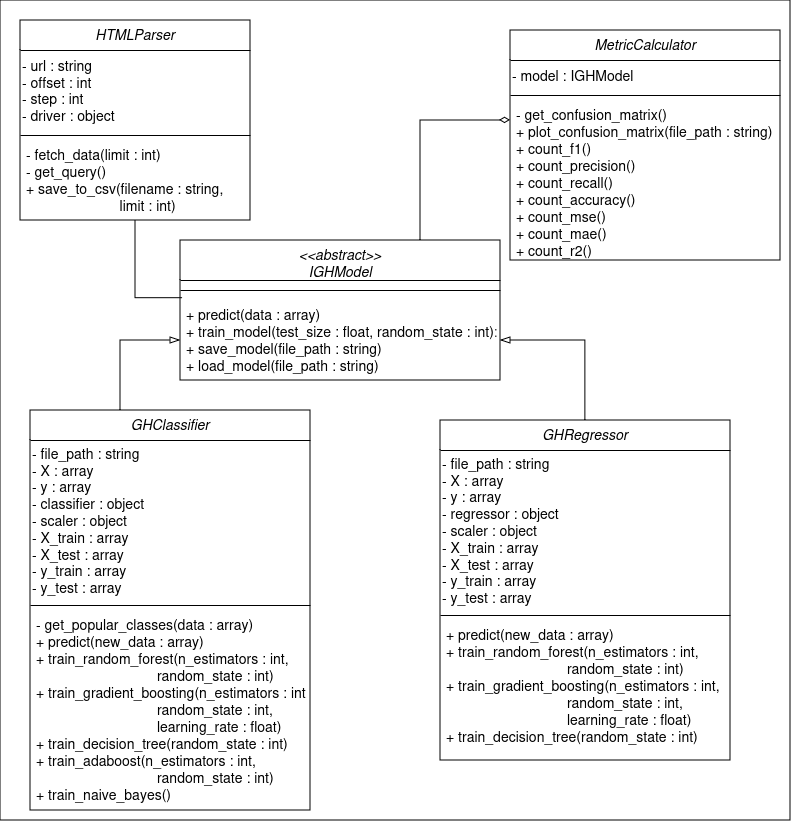
\includegraphics[width=1\linewidth]{pic/uml.png}
    \vspace{-0.5em}    \caption{Диаграмма классов UML}
    \label{ris:uml}
\end{figure}
\vspace{1em}

\subsection{Реализация пользовательского интерфейса}

Реализация пользовательского интерфейса осуществлялась на основе разработанных макетов. Реализованы главной страницы, страницы с вводом параметров и страницей результатов. В качестве основы разработки интерфейса использовалась библиотека Flask~\cite{flask}.

Главная страница (рис.~\ref{ris:main}) содержит приветственную форму с информацией о типах моделей и о том, что в результате можно получить. В данной форме содержится выпадающий список с выбором типа модели, где можно выбрать только один вариант для работы в дальнейшем, по умолчанию в данном списке всегда выбран вариант <<Модель классификации>>. При нажатии на кнопку <<Перейти>>  происходит переадресация на страницу в зависимости от выбора в списка.


Страница для определения класса популярности и страница для прогнозирования значения звезд репозитория имеют минимальные отличия. На рисунке~\ref{ris:input} представлена страница с вводом параметров для определения класса популярности проекта. 

\begin{figure}[h]
    \centering
    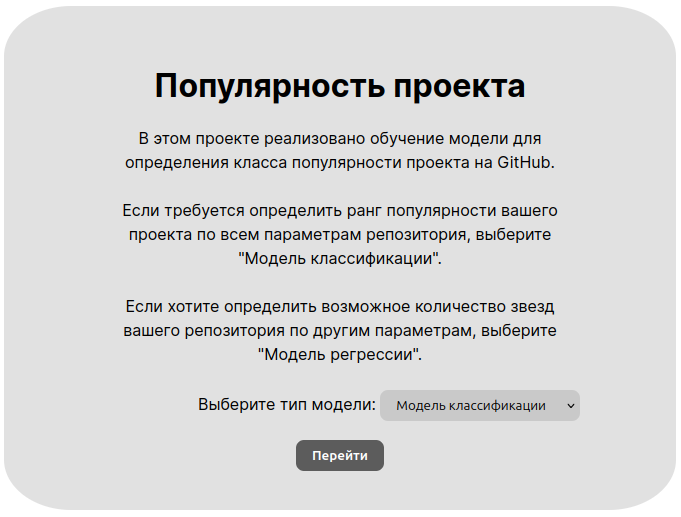
\includegraphics[width=1\linewidth]{pic/main.png}
    \vspace{-0.5em}    \caption{Форма на главной странице}
    \label{ris:main}
\end{figure}
\vspace{1em}

Для каждого параметра имеется свое поле для ввода, где название может содержать различные символы, а значение форков, звезд, проблем, коммитов, пулл-реквестов, участников -- только целочисленное значение. Все поля в данной форме обязательны для заполнения, при этом в случае отсутствия заполнения нет возможности узнать класс популярности. Внизу формы содержится выбор моделей классификации из тех, что показали самые лучшие результаты в метриках, по умолчанию в данном выпадающем списке стоит значение <<Градиентный бустинг>>. При нажатии на кнопку <<Узнать класс>> выполняется получение значения с помощью модуля классификации, после чего открывается страница с результатом. Страница для прогнозирования значения звезд отличает от данной отсутствием поля <<звезды>>.

\begin{figure}[h]
    \centering
    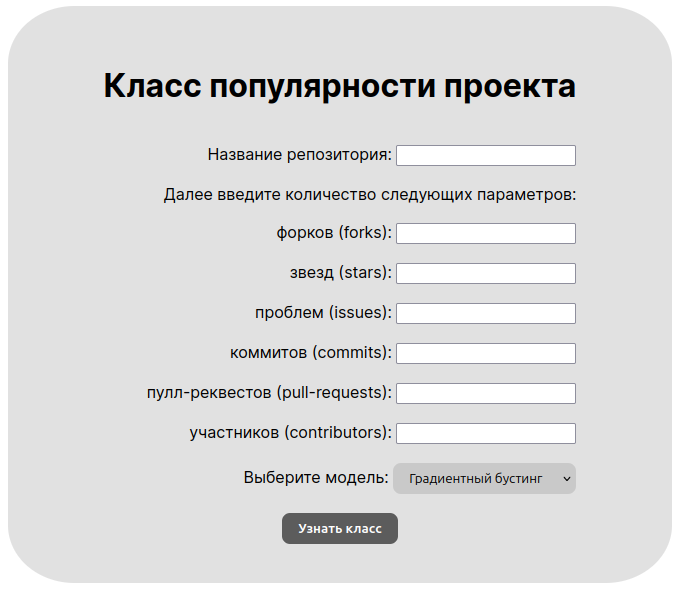
\includegraphics[width=1\linewidth]{pic/input.png}
    \vspace{-0.5em}    \caption{Форма на странице определения популярности}
    \label{ris:input}
\end{figure}
\vspace{1em}

Страница с результатами для определения класса популярности или звезд также имеют минимальные отличия. На рисунке~\ref{ris:result} представлен результат выполнения определения репозитория к классу.

На страницу приходит GET-запрос в котором содержатся данные для вывода результатов. Сама форма содержит строку с текстом, в котором содержится значение класса от 0 до 10 с пояснением о границах интервалов популярности. Поскольку результат может сильно отличаться о разных моделях также идет информация о ней. Кроме того, ниже перечислена введенная ранее пользователем информация для подтверждения того, что текущий результат получен именно от этих данных.

\begin{figure}[H]
    \centering
    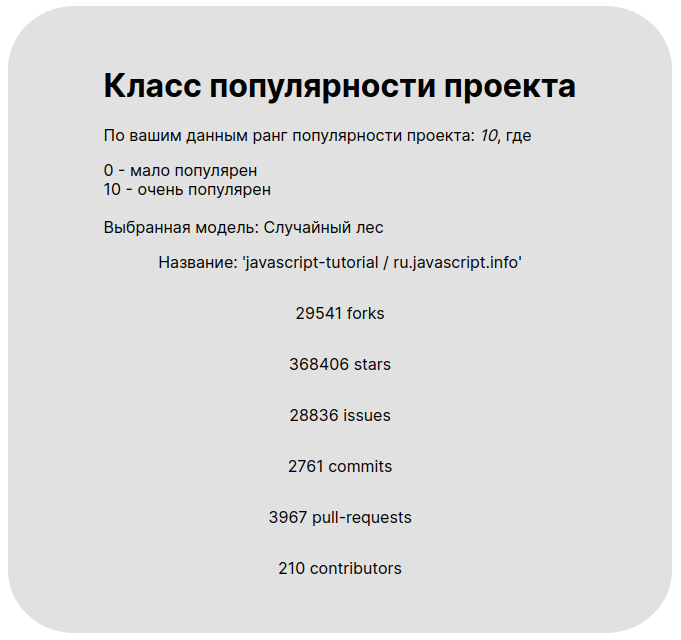
\includegraphics[width=1\linewidth]{pic/result.png}
    \vspace{-0.5em}    \caption{Форма на странице результатов}
    \label{ris:result}
\end{figure}
\vspace{1em}